%!TEX root = ../MasterThesis.tex

\section{Computer-Supported Cooperative Work}
\label{sec:cscw}

This section gives a short introduction to the theoretical foundations of \gls{CSCW} systems. It starts with an overview of the research field itself, followed by a description of the types of \gls{CSCW} systems available. After that it explains the concept of shared information spaces in detail.

\subsection{Fundamental aspects}
\label{sec:cscw_definition}

\gls{CSCW} is ``a \emph{generic} term which combines the understanding of the way people work in groups with the enabling technologies of computer networking, and associated hardware, software, services and techniques'' \citep[pg. 92]{borghoff2000computer}. It is part of the research field of \emph{Cooperation Systems}, which emerged during the early 1980s with the understanding that a multi-disciplinary approach for designing \gls{IT} systems is needed for the success of such systems. As such the research field looks into the usage of applications to support group work in an organizational setting, the effects of such a system on individual users, as well as how the applications have to be adapted for the context of the group. Therefore the studies of Cooperation Systems are consisting of a \emph{social} part as well as a \emph{technical} part, and are looking into the interrelationship between them for certain aspects of work in general, and explicitly for communication and cooperation in a team \citep{Grudin1994}. \\

These systems are generally focused on the concept of human-centered computing that wants to establish technology and work methods to improve processes and results of the work, while also improving the human conditions at work. A ``work system'' in such a sense describes the process of human work that consists of goal-directed activities in a \emph{professional} context. As more work has been moved to information workers another important aspect of such a system is the human cognition, which results in a need of taking human behavior as well as individual goals and knowledge into consideration. Therefore ``work systems'' focus on activities that is done by a group of people, a team, an organization or a society, and includes social factors like knowledge, goals, tasks and work of individuals or subgroups. These ``work systems'' are getting more and more complex as the problems human have to deal with are getting more difficult; in terms of their dynamic, nonlinear, interactive and simultaneous nature. Therefore humans have to continually adapt, take over different roles, and are engaged in various activities, which include management of the technologies used and handle the issues they introduce \citep{Hoffmann2009}. \\

That said a ``work system'' in this sense has two possible outcomes: the products and services created together by humans and/or machines and the sociological and psychological consequences as a result of being part of the process. The objective of a \emph{sociotechnical system} is to optimize both outcomes (see Figure~\ref{fig:images_sociotechnical_system}). \@

\begin{figure}[H]
  \centering
  \includegraphics[width=0.9\columnwidth]{images/sociotechnical_system.png}
  \caption[A sociotechnical work system]{A sociotechnical work system \citep{xx}}
  \label{fig:images_sociotechnical_system}
\end{figure}

To sum up \emph{sociotechnical} refers to the interrelatedness of social and technical aspects of an organization. The sociotechnical theory is founded on two main principles \citep{Koch2008}: \@

\begin{itemize}
  \item The interaction of social and technical factors creates the conditions for successful organizational performance. This interaction consists partly of linear ``cause and effect'' relationships and partly from ``non-linear'', often unpredictable relationships. Whether designed or not, both types of interaction occur when socio and technical elements are put to work.
  \item An optimization of each aspect alone (socio or technical) tends to increase not only the quantity of unpredictable relationships, but those relationships are injurious to the system's performance.
\end{itemize}

The success of a collaborative system depends highly on the level of active use of the system by its users. To improve the situation the system has to offer a clear balance between efforts and benefits for all of its users, has to communicate those to the users, and require a user-centered user interface as well as good integration into the user context \citep{Koch2008}.

% section cscw_defintion (end)

\subsection{Classification of \gls{CSCW} systems}
\label{sec:cscw_types}

In general \gls{CSCW} system can be classified based on the type of communication they support, the kind of applications they made possible as well as according to the ``3C model''. \\

In a distributed team environment the style of communication could be \emph{synchronous} or \emph{asynchronous} depending on the dimension of time. If the communication takes place at the same time the communication is synchronous, otherwise asynchronous. Another aspect that needs to be taken into account is the place. The team can be either co-located or geographically dispersed, which have a huge impact on the type of communication suitable. Taking both dimensions into account leads to the quadrant shown in Figure~\ref{fig:images_cscw_time_place_matrix}. \\

\begin{figure}[!ht]
 \centering
 \includegraphics[width=0.9\columnwidth]{images/time_place_matrix.png}
 \caption[Time/Place Matrix]{Time/Place Matrix \citep{robert2005paradox}}
\label{fig:images_cscw_time_place_matrix}
\end{figure}

Additionally it is possible to group the \gls{CSCW} systems based on the ``3C model'' into \citep[pg. 125]{borghoff2000computer}:

\begin{itemize}
  \item \textbf{communication:} a two way exchange of information between different team members,
  \item \textbf{coordination:} management of shared resources such as meeting rooms, network printers, file shares, \ldots,
  \item \textbf{collaboration:} members of a group work together in a shared environment to reach a predefined goal.
\end{itemize}

\begin{figure}[H]
 \centering
 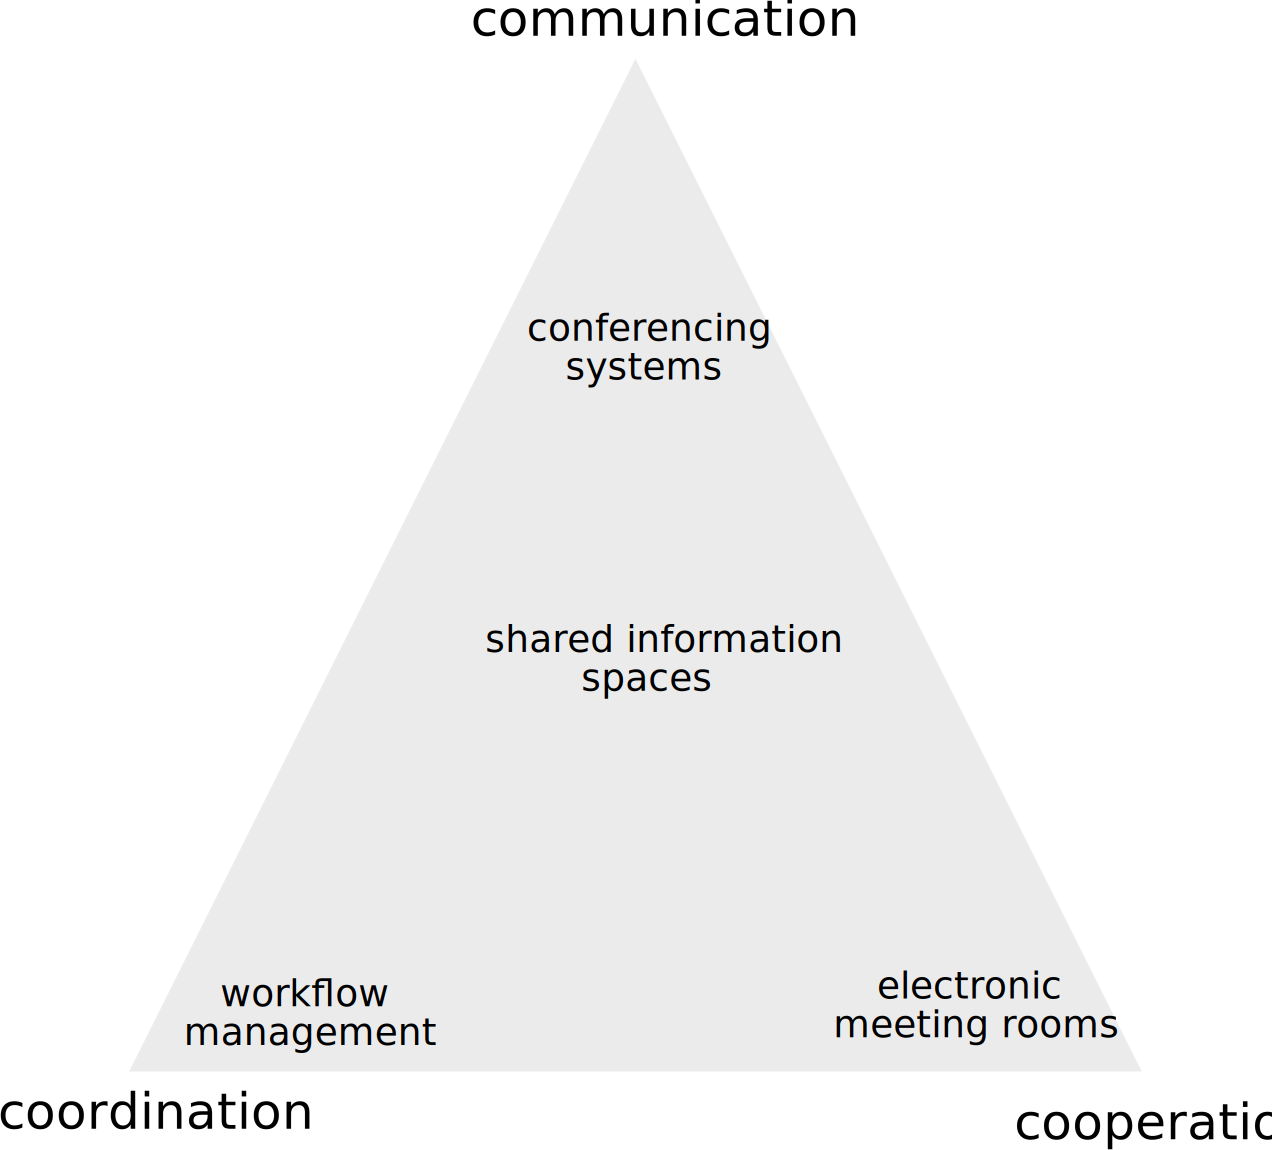
\includegraphics[width=0.9\columnwidth]{images/3C-model.png}
 \caption[The 3C Model]{The 3C Model \citep{Koch2008}}
\label{fig:images_cscw_3C_model}
\end{figure}

Typical application classes for \gls{CSCW} systems might be \citep[pg. 119-120]{borghoff2000computer}: \@

\begin{itemize}
  \item \textbf{message systems:} allow to exchange textual messages between team members asynchronously; modern systems include sending of other digital artefacts such as images and documents as well (e.g.\ instant messengers such as Microsoft Skype or Slack),
  \item \textbf{group editors:} allow collaborated work on some kind of shared document or artifact; editing of the shared document can be either allowed synchronously at the same time, or also asynchronously at different times (e.g.\ collaborative word processors such as Microsoft Word Online or Google Docs),
  \item \textbf{electronic meeting rooms:} allow multiple participants to work within a shared workspace or on a shared whiteboard, and offer support for ad-hoc brainstorming, idea generation and group decision making,
  \item \textbf{shared information spaces:} allow participants to access information at any place any time as well as to share information with others (e.g.\ Microsoft Sharepoint)
\end{itemize}

% section cscw_types (end)

\subsection{Shared Information Spaces}
\label{sec:cscw_shared_spaces}

In a \gls{CSCW} system shared information can take over two important roles: on the one hand they can transfer knowledge and facts between participants and on the other hand they resemble intermediate and final results of the group works themselves. In case of business critical information the system also have to provide a log of activities as well as a history of all artifacts generated or manipulated with them over time \citep[pg. 295]{borghoff2000computer}. \\

The kind of artifacts that are shared within such as collaborative system is not further specified, and can range from information, events or object representations from the real world to internal terms or objects of the working group. Whereas the former can be described extensively and usually do not need further interpretation, the latter one will need an interpretative component to define and clarify their intended meanings between group members. This common interpretation of terms and objects is even more important if the collaborative system is working across time and space boundaries, because co-located group member are generally having the same understanding of terms and objects due to being in the same (working) context and environment. Based to this fact, information that has to be shared between dispersed group members have to be refined and packaged in a way that enable the receiver to ``unpack'' the information and be able to re-create the original context, in which the information was created. Therefore the information in such a system is not just coming from a shared database, but also involves the joined interpretation of it by the actors involved \citep{bannon1997constructing}. \\

If information from different sources come together in a shared information space the collaborative system should support a nonlinear, exploratory way to retrieve and navigate through the information space to enable participants to browse and ascertain the concepts and their relations individually. A valid proposal for such a system is based on \emph{Hypertext}, because of its generic approach for the construction of nonlinear, computer-supported material that users can display and navigate on their screen in a nonlinear fashion. Hypertext systems are providing information that is distributed over a network of nodes, which make up the information space. Therefore, the information is divided into small, logical information units (aka nodes), in which references (aka links) are pointing to relevant or related units from the shared information space (see Figure~\ref{fig:images_cscw_hypertext_concept}). Users can navigate the information space along these links. A Hypertext system consists of three layers \citep[pg. 295-307]{borghoff2000computer}: \@

\begin{itemize}
  \item \textbf{database layer:} persists and manages the Hypertext information in a way that allows fast access and retrieval of information units,
  \item \textbf{Hypertext abstract machine:} creates an information network from the information units and their relations (aka links between them),
  \item \textbf{presentation:} displays individual information units on screen and allows the user to navigate the information space (via the links)
\end{itemize}

\begin{figure}[H]
 \centering
 
\includegraphics[width=0.9\columnwidth]{images/Hypertext.pdf}
 \caption[Example for a link between two nodes]{Example for a link between two nodes \citep[pg. 303]{borghoff2000computer}}
\label{fig:images_cscw_hypertext_concept}
\end{figure}

% section cscw_shared_spaces (end)

% section cscw (end)
